\chapter{Arduino}\label{analysis:arduino}
Arduino was created by the Interaction Design Institute Ivrea (Italy), by Massimo Banzi and David Cuartielles. They were looking for an easy and cheap way for students, who study design, to integrate micro controllers into their projects\cite{arduino:hist}. Both the board and the programming language was based on the works of Hernando Barragán, one of Massimo Banzi master thesis students \cite{Wiring:thesis}

\section{The hardware components}
Arduino is a single-board micro-controller, see figure \ref{fig:Arduino}.
A board consists of open source hardware, which is designed around an 8-bit Atmel AVR micro-controller. Arduino boards varies in sizes. Arduino Uno board for example, has a max width of 2.1'' (5,33cm) and a length of 2.7'' (6,86cm).  \\

\par
\raisebox{-.5\height}{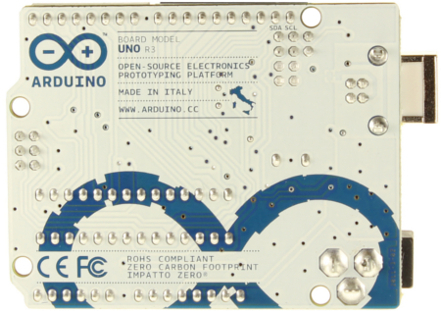
\includegraphics[width=6.5cm]{billeder/ArduinoUno_R3_Back_450px.jpg}}
\hfill
\raisebox{-.5\height}{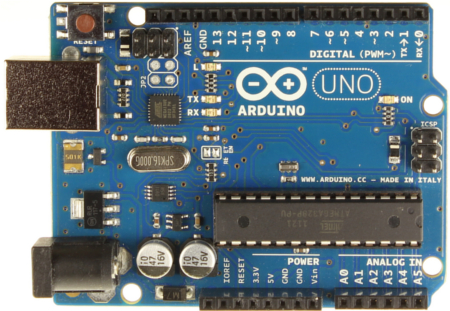
\includegraphics[width=6.5cm]{billeder/ArduinoUno_R3_Front_450px.jpg}}
\begin{figure}[H]
\caption{Picture of back- and fronside of the Arduino board \cite{Arduino_board_pics}}
\label{fig:Arduino}
\end{figure}
\par

The board provides some input and output possibilities. However these vary depending on the board, though most have 14 digital I/O and 6 analog inputs. The I/O functions are placed on top of the board, are freely accessible, and consist of 0.1'' female headers. Besides the I/O there is also a Power connector, which almost in all cases require 5 volt DC. There is a USB connection on the board, so that processing data to the micro-controller is possible, though it is shown as a virtual com-port on the connected computer. However, on older boards, instead of the USB connection, a RS232 were used for serial communication. 

On the board there is a LED diode which is connected to the digital pin 13. When this diode is set to ``HIGH'' it will be turned on, and if its value is ``LOW'' it turns off. Besides the LED diode, there is also a reset button. If the button is pressed the micro-controller is reset. 

Now what makes Arduino such a good platform for beginners to learn to code, is the fact that it is really easy to hook up the Arduino platform, to a wide array of components, to make it possible for the Arduino to interact with the real world.

\begin{tabular}{|l|l|}
\hline 
LED's & They come in all size, shapes and colors, ranging from small pin \\
& size single color LED's, to large multi color led displays.\\ 
\hline 
Sensors & These are some of the main components behind the Arduino\\
& success, they give the Arduino the ability to sense its surroundings,\\
& for instance the temperature of the room, whether the light is turn on,\\
& even advanced sensors like humidity or gas.  \\ 
\hline 
Motors & They give the Arduino the ability to manipulate its surrounding,\\
& and act on the informations obtained from the sensors. There are two kind \\
& of motors, normal motors which can just be turned on/off, they are great \\
& for powering wheels or tracks to allow it to move. There are stepper motors \\
& with it is possible to control the exact amount of rotation. And finally \\
& there is servos, which are precisely controlled motors much like the stepper motor,\\
&  but much more precise.  \\
\hline 
Displays & There are a wide range of display available ranging from\\ 
& simple 2 line mono color LCD displays, all the way up to large\\
& OLED color and touch displays.   \\ 
\hline 
Communication & It is easy to hook up the Arduino with some form\\ & of communication allowing it to communicate with other devices\\
& either through, RF signals, bluetooth, WiFi, cellular or just\\
& plain old Ethernet connection \\ 
\hline 
Shields & Finally the last thing which makes the Arduino great is it modularity,\\
& in the form of shields. Shields are boards much like the Arduino it self,\\
& but they offer all the capabilities of the components mentioned above, \\
& but they do it in a way, which makes it possible for any one with \\
& out any electronics experience to use them, you just plug the shield \\
& on top of the Arduino board, and all the components need to are included. \\
\hline
\end{tabular} 

